\documentclass[10pt,pdf,utf8,russian,aspectratio=169]{beamer}
\usepackage{cmap}
\usepackage[T2A]{fontenc}
%\usepackage[utf8x]{inputenc}
\usepackage[russian,english]{babel}
\usepackage{subfig}
\usepackage{graphicx}
\usepackage{multicol}
\usepackage{cancel}
\usepackage{tabularx}
\usepackage{xargs}      
\usepackage{mathbbol}
\usepackage{amssymb}  
\usepackage{tikz} 
\DeclareSymbolFontAlphabet{\mathbb}{AMSb}%
\DeclareSymbolFontAlphabet{\amsmathbb}{bbold}%
\DeclareUnicodeCharacter{00A0}{ } % При наборе текста с планшета появляются невидимые символы. ЭТо костыль.

\usetikzlibrary{arrows,automata}
\usetikzlibrary{positioning}


       % AMS Math

%
% Choose how your presentation looks.
%
% For more themes, color themes and font themes, see:
% http://deic.uab.es/~iblanes/beamer_gallery/index_by_theme.html
%
\mode<presentation>
{
  \usetheme{Boadilla}      % or try Darmstadt, Madrid, Warsaw, ...
  \usecolortheme{seagull} % or try albatross, beaver, crane, ..

  \usefonttheme{structurebold}  % or try serif, structurebold, ...
  \setbeamertemplate{navigation symbols}{}
  \setbeamertemplate{caption}[numbered]
} 

\captionsetup[subfloat]{labelformat=empty}
\title[Структура]{Выбор структуры модели глубокого обучения}
\author{Бахтеев Олег}
\institute{МФТИ}
\date{20.11.2019}
%\renewcommand{\headrulewidth}{0pt}
\DeclareMathOperator*{\argmin}{arg\,min}
\DeclareMathOperator*{\argmax}{arg\,max}
\DeclareUnicodeCharacter{00A0}{ } % При наборе текста с планшета появляются невидимые символы. ЭТо костыль.
\begin{document}
% nb: очень не люблю макросы. Но что поделать 
% https://stackoverflow.com/questions/1509799/how-to-replace-latex-macros-with-their-definitions-using-latex
\newcommand{\D}{\mathfrak{D}}
\newcommand{\x}{\mathbf{x}}
\newcommand{\X}{\mathbf{X}}
\newcommand{\y}{\mathbf{y}}
\newcommand{\Xb}{\mathbb{X}}
\newcommand{\yb}{\mathbb{Y}}
\newcommand{\F}{\mathfrak{F}}



\newcommand{\w}{\mathbf{w}}
\newcommand{\Wb}{\mathbb{W}}
\newcommand{\Uw}{U_\mathbf{w}}

\newcommand{\Gam}{\boldsymbol{\Gamma}}
\newcommand{\Gb}{\amsmathbb{\Gamma}}
\newcommand{\UG}{U_{\boldsymbol{\Gamma}}}

\newcommand{\h}{\mathbf{h}}
\newcommand{\Hb}{\mathbb{H}}
\newcommand{\Uh}{U_{\mathbf{h}}}

\newcommand{\teta}{\boldsymbol{\theta}}
\newcommand{\Tetab}{\amsmathbb{\Theta}}
\newcommand{\Uteta}{U_{\boldsymbol{\theta}}}

\newcommand{\tetaw}{\boldsymbol{\theta}_\mathbf{w}}
\newcommand{\Tetawb}{\amsmathbb{\Theta}_\mathbf{w}}
\newcommand{\Utetaw}{U_{\boldsymbol{\theta}_\mathbf{w}}}
\newcommand{\tetaG}{\boldsymbol{\theta}_{\boldsymbol{\Gamma}}}
\newcommand{\TetaGb}{\amsmathbb{\Theta}_{\boldsymbol{\Gamma}}}
\newcommand{\UtetaG}{U_{\boldsymbol{\theta}_{\boldsymbol{\Gamma}}}}

\newcommand{\lam}{\boldsymbol{\lambda}}
\newcommand{\Lamb}{\amsmathbb{\Lambda}}
\newcommand{\Ulam}{U_{\boldsymbol{\lambda}}}

%\newcommand{\prior}{p(\mathbf{w}, \boldsymbol{\Gamma}|\mathbf{h},\boldsymbol{\lambda})}
\newcommandx{\prior}[4][1=\mathbf{w},2=\boldsymbol{\Gamma},3=\mathbf{h},4=\boldsymbol{\lambda},usedefault]{p(#1,#2|#3,#4)}
\newcommandx{\priorh}[2][1=\mathbf{h}, 2=\boldsymbol{\lambda},usedefault]{p(#1|#2)}
\newcommandx{\priorG}[3][1=\boldsymbol{\Gamma}, 2= \mathbf{h}, 3=\boldsymbol{\lambda},usedefault]{p(#1|#2,#3)}
\newcommandx{\priorw}[4][1=\mathbf{w},2=\boldsymbol{\Gamma},3=\mathbf{h},4=\boldsymbol{\lambda},usedefault]{p(#1|#2,#3,#4)}


\newcommand{\post}{p(\mathbf{w}, \boldsymbol{\Gamma}|\mathbf{y}, \mathbf{X}, \mathbf{h},\boldsymbol{\lambda})}
\newcommand{\posth}{p(\mathbf{h}|\mathbf{y}, \mathbf{X},\boldsymbol{\lambda})}
\newcommand{\postG}{p(\boldsymbol{\Gamma}|\mathbf{y}, \mathbf{X}, \mathbf{h},\boldsymbol{\lambda})}
\newcommand{\postw}{p(\mathbf{w}|\mathbf{y}, \mathbf{X}, \boldsymbol{\Gamma}, \mathbf{h},\boldsymbol{\lambda})}


\newcommandx{\q}[1][1=\boldsymbol{\theta}, usedefault]{q(\mathbf{w}, \boldsymbol{\Gamma}|#1)}
\newcommandx{\qG}[2][1=\boldsymbol{\Gamma},2=\boldsymbol{\theta}_{\boldsymbol{\Gamma}},usedefault]{q_{\boldsymbol{\Gamma}}(#1|#2)}
\newcommandx{\qw}[3][1=\mathbf{w}, 2=\boldsymbol{\Gamma},3=\boldsymbol{\theta}_\mathbf{w},usedefault]{q_\mathbf{w}(#1|#2,#3)}


\newcommandx{\LL}[4][1=\mathbf{y},2=\mathbf{X},3=\mathbf{w},4=\boldsymbol{\Gamma},usedefault]{p(#1|#2,#3,#4)}

\newcommand{\EV}{p(\mathbf{y}|\mathbf{X}, \mathbf{h},\boldsymbol{\lambda})}

\newcommandx{\Loss}[5][1=\boldsymbol{\theta},2=\mathbf{y},3=\mathbf{X},4=\mathbf{h},5=\boldsymbol{\lambda},usedefault]{L(#1 |#2,#3,#4,#5)}
\newcommandx{\Val}[5][1=\mathbf{h},2=\mathbf{y},3=\mathbf{X},4=\boldsymbol{\theta},5=\boldsymbol{\lambda},usedefault]{Q(#1|#2,#3,#4,#5)}

% прочее
\newcommand{\model}{\mathbf{f}}
\newcommand{\A}{\mathbf{A}}
\newcommand{\s}{\mathbf{s}}
\newcommand{\g}{\boldsymbol{\gamma}}
\newcommand{\E}{\mathsf{E}}
\newcommand{\KL}[2]{D_\text{KL}\bigl(#1 || #2\bigr)}

\newcommand{\lamT}{\lambda_{\text{temp}}}
\newcommand{\lamLL}{\lambda_\text{likelihood}^\text{Q}}
\newcommand{\lamCL}{\lambda_\text{prior}^\text{L}}
\newcommand{\lamCQ}{\lambda_\text{prior}^\text{Q}}
\newcommand{\lamS}{\boldsymbol{\lambda}_\text{struct}^\text{Q}}
\newcommandx{\TLoss}[6][1=\boldsymbol{\theta},2=L,3=\mathbf{y}, 4=\mathbf{X}, 5=\mathbf{h},6=\boldsymbol{\lambda},usedefault]{T(#1|#2,#3,#4,#5,#6)}
\newcommandx{\TVal}[6][1=\mathbf{h},2=Q,3=\mathbf{y}, 4=\mathbf{X}, 5=\boldsymbol{\teta},6=\boldsymbol{\lambda},usedefault]{T(#1|#2,#3,#4,#5,#6)}
%\newcommand{\log}{\text{log}~}




\begin{frame}
  \titlepage
\end{frame}

\begin{frame}{Резюме прошлых семинаров}
\textbf{Заданы: }
\begin{itemize}
\item Вариационное распределение $\qw$ с параметрами $\teta$;
\item Априорное распределение $\priorw$ с параметрами $\h$;
\item Функция потерь $L$ и функция валидации $Q$.
\end{itemize}
\vspace{0.2cm}
\textbf{Требуется:} предложить метод выбора структуры модели $\Gam$.\\
\vspace{0.2cm}
\textbf{Вопросы:}
\begin{itemize}
\item Как задать структуру модели?
\item Как провести ее выбор?
\item Какова вероятностная интерпретация структуры?
\end{itemize}

\end{frame}

\begin{frame}{Automatic relevance determination}
\textbf{Идея:} при оптимизации Evidence \textit{априорное} распределение неинформативных параметров будет сконцентрировано в нуле:
\[
    \w \sim \mathcal{N}(0, \mathbf{A}), \quad \mathbf{A}=\text{diag}(\boldsymbol{\alpha}).
\]
$w_i$ --- неинформативен $\rightarrow \alpha_i \approx 0.$
\vspace{1cm}

\textbf{Параллель с вариационным выводом:}
прунинг параметра ${w}_i$ определяется относительной плотностью:
\[
	\lambda = \frac{q(\mathbf{0})}{q(\boldsymbol{\mu}_{i,q})}  = \text{exp}(-\frac{\mu_i^2}{2\sigma_i^2}).
\]
\end{frame}

\begin{frame}{Пример: вариационный автокодировщик + ARD}
\begin{columns}[T] 
\begin{column}{.48\textwidth}
\textbf{VAE:}
\[
    L = \int_{\mathbf{z}} p(\x|\mathbf{z})p(\mathbf{z})d\mathbf{z}.
\]

\textbf{VAE + ARD:}
\[
    L = \iint_{\mathbf{z}, \boldsymbol{\gamma}} p(\x|\mathbf{z} \odot \boldsymbol{\gamma})p(\mathbf{z})p(\boldsymbol{\gamma})d\mathbf{z}d\boldsymbol{\gamma}.
\]
\end{column}
\begin{column}{.48\textwidth}

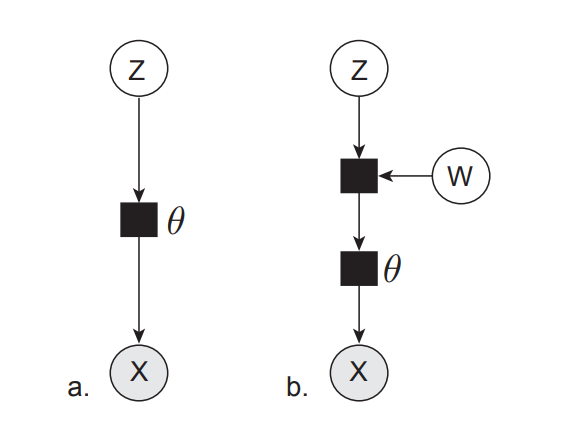
\includegraphics[width=\textwidth]{ard_vae.png}
\end{column}
\end{columns}

\end{frame}


\begin{frame}{AdaNet}
\begin{columns}[T] 
\begin{column}{.48\textwidth}
В качестве алгоритма выбора структуры модели выступает бустинговый алгоритм.

На каждом шаге бустинга рассматривается две альтернативы: добавить новую слабую модель той же глубины или более глубокую.

Оптимизируемый функционал:
\[
    Q = \sum_{i} \Phi(1- y_i f_{t-1}\left(\mathbf{x}_i)  - y_i \boldsymbol{\gamma}' f'(\mathbf{x})\right) + \mathcal{R},
\]
где $\mathcal{R}$ --- оценка сложности по Радемахеру.
\end{column}
\begin{column}{.48\textwidth}
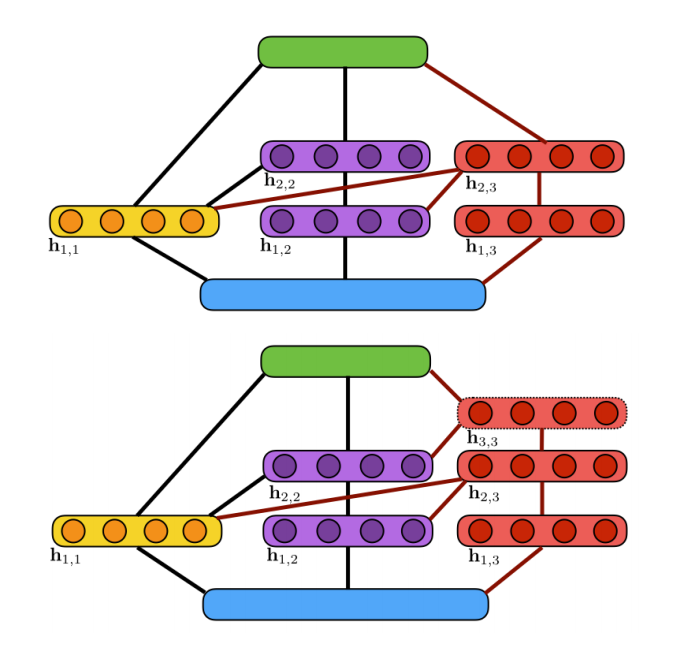
\includegraphics[width=\textwidth]{adanet.png}
\end{column}
\end{columns}
\end{frame}


\begin{frame}{Neural Architecture Search}
\begin{columns}[T] 
\begin{column}{.48\textwidth}
\textbf{Идея алгоритма:} модели порождаются с использованием обучения с подкреплением. Контроллер - рекуррентная нейронная сеть.

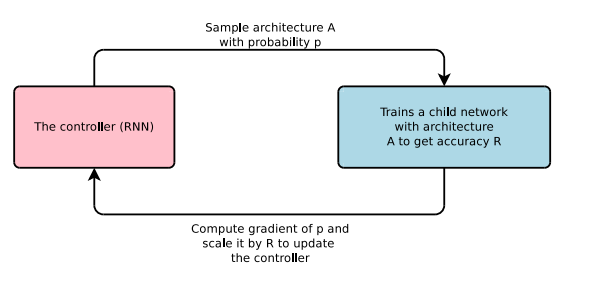
\includegraphics[width=\textwidth]{nas_scheme.png}
\end{column}
\begin{column}{.48\textwidth}
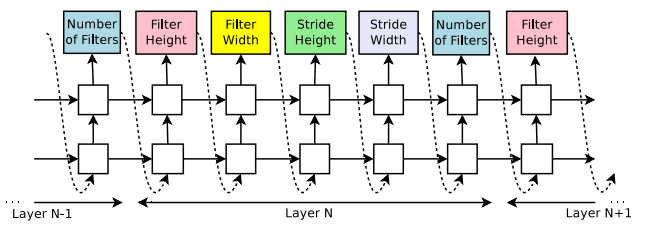
\includegraphics[width=\textwidth]{nas_seq.png}
\end{column}
\end{columns}
\end{frame}


\begin{frame}{Neural Architecture Search}
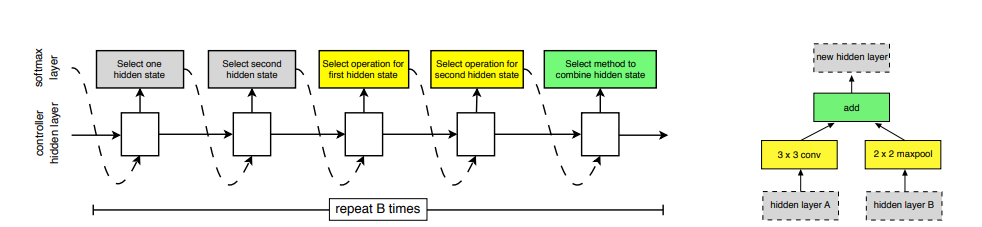
\includegraphics[width=\textwidth]{nas_transfer.png}

Для оптимизации использовалось 500 GPU.
\end{frame}


\begin{frame}{Neural Architecture Search: результаты}

\begin{figure}
  \centering
 {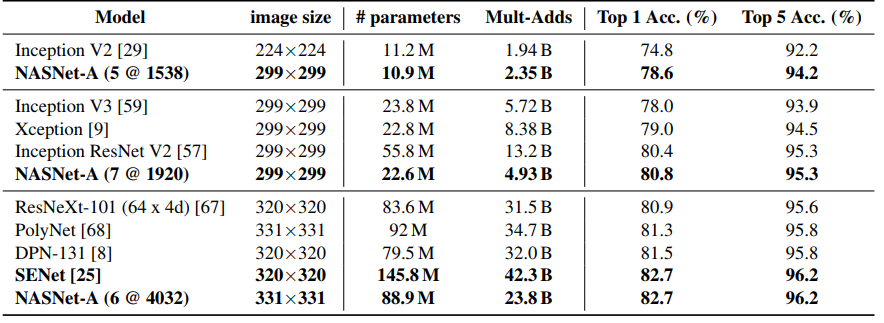
\includegraphics[width=\textwidth]{zoph.png}}
\label{fig:1}\qquad
\caption*{Zoph et al., 2017.  Сложность моделей отличается почти в два раза при одинаковом качестве.}
\end{figure}

\end{frame}

\begin{frame}{Neural Architecture Search: постановка задачи}
$\w$ (или $\qw$) --- параметры модели, оптимизируемые при заданной структуре.

$\Gam$ (или $\qG$) --- структура модели, задается контроллером, должна доставлять максимум валидации.

\[
    \Gam^{*} = \argmax Q (\w^{*}, \Gam),
\]
\[
    \w^{*} = \argmax L(\w, \Gam).
\]

\textit{Нужно ли здесь обучение с подкреплением?}
\end{frame}

\begin{frame}{DARTS}
\begin{columns}[T] 
\begin{column}{.48\textwidth}
Модель --- мультиграф, где ребра $[\mathbf{g}^e]$ соответствуют подмоделям, а вершины $\mathbf{f}_v(\mathbf{x})$ --- результату действия подмоделей на выборку. 

Результат применения подмоделей:
\[
    \mathbf{f}_v = \langle\boldsymbol{\gamma}, \textbf{softmax}([\mathbf{g}^e (\mathbf{x})])\rangle.
\]
\end{column}
\begin{column}{.48\textwidth}
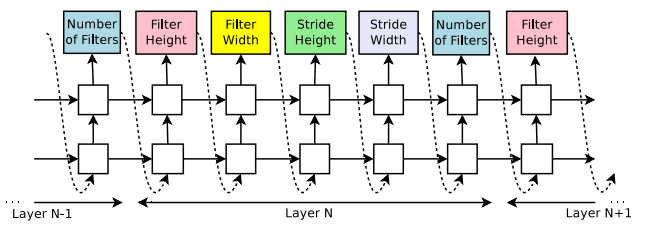
\includegraphics[width=\textwidth]{nas_seq.png}
\end{column}
\end{columns}
\end{frame}


\begin{frame}{DARTS}
Задача оптимизации:
\[
    \Gam^{*} = \argmax Q (\w^{*}, \Gam), Q \text{--- ошибка на валидации},
\]
\[
    \w^{*} = \argmax L(\w, \Gam), L \text{--- ошибка на обучении}.
\]

Оптимизация структуры производится жадным градиентным методом:
$$
    \nabla_{\Gam} Q( \w', \Gam) = \lambda_L \nabla_{\Gam, \w} L(\w, \Gam)\nabla_{\w}Q(\Gam, \w').
$$

\textit{Напоминание:}\\
Численное приближение аналитической формулы:
 \[\nabla_{\mathbf{h}}Q(\boldsymbol{\theta}^\eta, \mathbf{h}) - \nabla_{\mathbf{h}}\nabla_{\boldsymbol{\theta}} L(\boldsymbol{\theta}^\eta, \mathbf{h})^\text{T}\mathbf{H}^{-1}\nabla_{\boldsymbol{\theta}}Q(\boldsymbol{\theta}^\eta, \mathbf{h}).\]

Для быстрого вычисления множителя $\nabla_{\Gam, \w} L(\w, \Gam)$ используется метод конечных приращений.
\end{frame}



\begin{frame}{Графовое представление модели глубокого обучения}
\footnotesize
Заданы:
\begin{enumerate}
 \item ациклический граф $(V,E)$;
\item для каждого ребра $(j,k) \in E$: вектор базовых дифференцируемых функций  $\mathbf{g}^{j,k} = [\mathbf{g}^{j,k}_0, \dots, \mathbf{g}^{j,k}_{K^{j,k}}]$  мощности $K^{j,k}$;
\item для каждой вершины $v \in V$: дифференцируемая функция агрегации $\textbf{agg}_v$.
\item Функция $\mathbf{f} = \mathbf{f}_{|V|-1}$, задаваемая по правилу 
\begin{equation}
\label{eq:modelfam}
    \mathbf{f}_{v}(\mathbf{w}, \mathbf{x}) = \textbf{agg}_{v}\left(\{ \langle \boldsymbol{\gamma}^{j,k}, \mathbf{g}^{j,k} \rangle \circ  \mathbf{f}_j(\mathbf{x})| j \in \text{Adj}(v_k)\}\right), v \in \{1,\dots,|V|-1\}, \quad \mathbf{f}_0(\mathbf{x}) = \mathbf{x}
\end{equation}
и являющаяся функцией из признакового пространства $\mathbb{X}$ в пространство меток $\mathbb{Y}$ при значениях векторов, $\boldsymbol{\gamma}^{j,k} \in [0,1]^{K^{j,k}}$.
\end{enumerate}

\begin{block}{Определение}
Граф $(V, E)$ со множестом векторов базовых функций $\{\mathbf{g}^{j,k}, (j,k) \in E\}$ и функций агрегаций $\{ \textbf{agg}_v, {v \in V}\}$ назовем \textit{параметрическим семейством моделей} $\mathfrak{F}$.
\end{block}
\begin{block}{Утверждение}
Для любого значения $\boldsymbol{\gamma}^{j,k} \in [0,1]^{K^{j,k}}$ функция $\mathbf{f} \in \mathfrak{F}$ является моделью.
\end{block}
\end{frame}


\begin{frame}{Выбор структуры: двуслойная нейросеть}
\small
Модель $\mathbf{f}$ задана \textbf{структурой}  $\boldsymbol{\Gamma} = [\boldsymbol{\gamma}^{0,1}, {\boldsymbol{\gamma}^{1,2}}].$

\[
    \text{Модель: }\mathbf{f}(\mathbf{x}) = \textbf{softmax}\left((\mathbf{w}^{1,2}_0)^\mathsf{T}{\mathbf{f}_1}(\mathbf{x})\right), \quad \mathbf{f}(\mathbf{x}): \mathbb{R}^n \to [0,1]^{|\mathbb{Y}|}, \quad \mathbf{x} \in \mathbb{R}^n.
\]
\[
\mathbf{f}_1(\mathbf{x}) = {\gamma}^{0,1}_{0}\mathbf{g}^{0,1}_{0}(\mathbf{x}) + {\gamma}^{0,1}_{1}\mathbf{g}^{0,1}_{1}(\mathbf{x}),
\]
где $\mathbf{w} = [\mathbf{w}^{0,1}_0, \mathbf{w}^{0,1}_1, \mathbf{w}^{1,2}_0]^{\text{T}}$ --- матрицы параметров, $\{\mathbf{g}^{0}_{0,1},\mathbf{g}^{1}_{0,1},{\mathbf{g}^{0}_{1,2}\}}$ --- обобщенно-линейные функции скрытых слоев нейросети.

\begin{tikzpicture}[node distance=0.5cm, auto]
  %\tikzstyle{every state}=[fill=red,draw=none,text=white]

  \node (f0)  at (1,6)                  {$\mathbf{f}_0(\mathbf{x}) = \mathbf{x}$};
  %\node (g11) at (6,3)                    {$\mathbf{g}^{1,1}(\mathbf{x})$};% = \text{Conv}(\mathbf{x}, 3, 32, 1)$};
  %\node (g12)  at (6,9)                   {$\mathbf{g}^{1,2}(\mathbf{x})$};% = \text{Conv}(\mathbf{x}, 4, 32, 1)$};
  \node (f1)  at (7,6)                 {$\mathbf{f}_1(\mathbf{x})$};% = \gamma^{1,1}\mathbf{g}^{1,1}(\mathbf{x}) +  \gamma^{1,2}\mathbf{g}^{1,2}(\mathbf{x})$};
  %\node (g21) at (12,6)                   {$\mathbf{g}^{2,1}(\mathbf{x})$};% = \boldsymbol{\sigma}(\mathbf{w}^{2,1}\mathbf{x})$};
  \node (f2)  at (12,6)                   {$\mathbf{f}_2(\mathbf{x})$};% = \gamma^{2,1}\mathbf{g}^{2,1}(\mathbf{x})$};
  \path[->]  (f0) edge [bend left=50] node {$\gamma^{0,1}_0\mathbf{g}^{0,1}_0(\mathbf{x}) = \gamma^{0,1}_0\boldsymbol{\sigma}\left((\mathbf{w}^{0,1}_0)^{\mathsf{T}}\mathbf{x}\right)$}(f1);
  \path[->] (f0)  edge[bend right=50] node[below] {$\gamma^{0,1}_1\mathbf{g}^{0,1}_1(\mathbf{x}) = \gamma^{0,1}_1\boldsymbol{\sigma}\left((\mathbf{w}^{0,1}_1)^{\mathsf{T}}\mathbf{x}\right)$}(f1);
  \path[->] (f1)  edge node {$\gamma^{1,2}_0\mathbf{g}^{1,2}_0(\mathbf{x}) = \gamma^{1,2}_0\textbf{softmax}\left((\mathbf{w}^{1,2}_0)^{\mathsf{T}}\mathbf{x}\right)$}(f2);       
  \draw[->] (f1) to (f2);
 
\end{tikzpicture}

\end{frame}





\begin{frame}{Ограничения на структурные параметры}
Примеры ограничений для одного структурного параметра $\boldsymbol{\gamma}, |\boldsymbol{\gamma}| = 3$.
\begin{figure}
 \begin{minipage}[t]{.45\textwidth}
        \centering
%1 limit
\begin{tikzpicture}[%
x={(1.5cm,0cm)},
y={(0cm,1.5cm)},
z={({0.5*cos(45)},{0.5*sin(45)})},
]

\coordinate (A) at (0,0,0); 
\coordinate (B) at (1,0,0) ;
\coordinate (C) at (1,1,0); 
\coordinate (D) at (0,1,0); 
\coordinate (E) at (0,0,1); 
\coordinate (F) at (1,0,1); 
\coordinate (G) at (1,1,1); 
\coordinate (H) at (0,1,1   );

%Ecken
\node[circle,scale=0.5,fill=black,draw=black](Ap) at (0,0,0){};
\node[circle,scale=0.5,fill=black,draw=black](Bp) at (1,0,0){};
\node[circle,scale=0.5,fill=black,draw=black](Cp) at (1,1,0){};
\node[circle,scale=0.5,fill=black,draw=black](Dp) at (0,1,0){};
\node[circle,scale=0.5,fill=black,draw=black](Ep) at (0,0,1){};
\node[circle,scale=0.5,fill=black,draw=black](Fp) at (1,0,1){};
\node[circle,scale=0.5,fill=black,draw=black](Gp) at (1,1,1){};
\node[circle,scale=0.5,fill=black,draw=black](Hp) at (0,1,1){};
\node[left= 1pt of A]{[0,0,0]};
\node[right= 1pt of B]{[1,0,0]};
\node[right= 1pt of C]{[1,1,0]};
\node[left= 1pt of D]{[0,1,0]};
\node[left= 1pt of E]{[0,0,1]};
\node[right= 1pt of F]{[1,0,1]};
\node[right= 1pt of G]{[1,1,1]};
\node[left= 1pt of H]{[0,1,1]};

%Kanten
\draw[] (A)
-- (B)  node[midway, below]{}
-- (C)      node[midway, right]{}
-- (D)  node[midway, above]{}
-- (A)  node[midway, left]{};
\draw[] (B) -- (F) -- (G) -- (C);
\draw[] (G) -- (H) -- (D);
\draw[densely dashed] (A) -- (E) -- (F);
\draw[densely dashed] (E) -- (H);

\end{tikzpicture}
\caption*{На вершинах куба}
\end{minipage}
\hfill
 \begin{minipage}[t]{.45\textwidth}
        \centering

%2 limit
\begin{tikzpicture}[%
x={(1.5cm,0cm)},
y={(0cm,1.5cm)},
z={({0.5*cos(45)},{0.5*sin(45)})},
]

\coordinate (A) at (0,0,0); 
\coordinate (B) at (1,0,0) ;
\coordinate (C) at (1,1,0); 
\coordinate (D) at (0,1,0); 
\coordinate (E) at (0,0,1); 
\coordinate (F) at (1,0,1); 
\coordinate (G) at (1,1,1); 
\coordinate (H) at (0,1,1   );

%Ecken
\node[left= 1pt of A]{[0,0,0]};
\node[right= 1pt of B]{[1,0,0]};
\node[right= 1pt of C]{};
\node[left= 1pt of D]{[0,1,0]};
\node[left= 1pt of E]{};
\node[right= 1pt of F]{[1,0,1]};
\node[right= 1pt of G]{[1,1,1]};
\node[left= 1pt of H]{[0,1,1]};

%Kanten
\draw[fill=gray] (A)
-- (B)  node[midway, below]{}
-- (C)      node[midway, right]{}
-- (D)  node[midway, above]{}
-- (A)  node[midway, left]{};
\draw[fill=gray] (B) -- (F) -- (G) -- (C);
\draw[fill=gray] (G) -- (H) -- (D);
\draw[fill=gray] (A) -- (E) -- (F);
\draw[fill=gray] (E) -- (H);
\draw[fill=gray] (D) -- (H) -- (G) -- (C);
\end{tikzpicture}
\caption*{Внутри куба}
\end{minipage}
\hfill
 \begin{minipage}[t]{.45\textwidth}
        \centering
%3 limit
\begin{tikzpicture}[%
x={(1.5cm,0cm)},
y={(0cm,1.5cm)},
z={({0.5*cos(45)},{0.5*sin(45)})},
]

\coordinate (A) at (0,0,0); 
\coordinate (B) at (1,0,0) ;
\coordinate (C) at (1,1,0); 
\coordinate (D) at (0,1,0); 
\coordinate (E) at (0,0,1); 
\coordinate (F) at (1,0,1); 
\coordinate (G) at (1,1,1); 
\coordinate (H) at (0,1,1   );

%Ecken
\node[circle,scale=0.5,fill=black,draw=black](Bp) at (1,0,0){};
\node[circle,scale=0.5,fill=black,draw=black](Dp) at (0,1,0){};
\node[circle,scale=0.5,fill=black,draw=black](Ep) at (0,0,1){};
\node[left= 1pt of A]{};
\node[right= 1pt of B]{[1,0,0]};
\node[right= 1pt of C]{};
\node[left= 1pt of D]{[0,1,0]};
\node[left= 1pt of E]{[0,0,1]};
\node[right= 1pt of F]{};
\node[right= 1pt of G]{};
\node[left= 1pt of H]{};

%Kanten
\draw[] (A)
-- (B)  node[midway, below]{}
-- (C)      node[midway, right]{}
-- (D)  node[midway, above]{}
-- (A)  node[midway, left]{};
\draw[] (B) -- (F) -- (G) -- (C);
\draw[] (G) -- (H) -- (D);
\draw[densely dashed] (A) -- (E) -- (F);
\draw[densely dashed] (E) -- (H);

\end{tikzpicture}
\caption*{На вершинах симплекса}
\end{minipage}
\hfill
 \begin{minipage}[t]{.45\textwidth}
        \centering
%4 limit
\begin{tikzpicture}[%
x={(1.5cm,0cm)},
y={(0cm,1.5cm)},
z={({0.5*cos(45)},{0.5*sin(45)})},
]

\coordinate (A) at (0,0,0); 
\coordinate (B) at (1,0,0) ;
\coordinate (C) at (1,1,0); 
\coordinate (D) at (0,1,0); 
\coordinate (E) at (0,0,1); 
\coordinate (F) at (1,0,1); 
\coordinate (G) at (1,1,1); 
\coordinate (H) at (0,1,1   );

%Ecken
\node[left= 1pt of A]{};
\node[right= 1pt of B]{[1,0,0]};
\node[right= 1pt of C]{};
\node[left= 1pt of D]{[0,1,0]};
\node[left= 1pt of E]{[0,0,1]};
\node[right= 1pt of F]{};
\node[right= 1pt of G]{};
\node[left= 1pt of H]{};

%Kanten
\draw[] (A)
-- (B)  node[midway, below]{}
-- (C)      node[midway, right]{}
-- (D)  node[midway, above]{}
-- (A)  node[midway, left]{};
\draw[] (B) -- (F) -- (G) -- (C);
\draw[] (G) -- (H) -- (D);
\draw[densely dashed] (A) -- (E) -- (F);
\draw[densely dashed] (E) -- (H);
\draw[fill=gray] (B) -- (D) -- (E);


\end{tikzpicture}
\caption*{Внутри симплекса}
\end{minipage}

\end{figure}

\end{frame}


\begin{frame}{Распределение Дирихле}
Каждая точка на симплексе задает модель.


\begin{figure}
 \begin{minipage}[t]{.3\textwidth}
        \centering
\begin{tikzpicture}[%
x={(1.7cm,0cm)},
y={(0cm,1.7cm)},
]

\coordinate (A) at (0,0); 
\coordinate (B) at (1,0) ;
\coordinate (C) at (0.5,0.86); 

%Ecken
\node[circle,scale=0.5,fill=black,draw=black](Ap) at (0,0){};
\node[circle,scale=0.5,fill=black,draw=black](Bp) at (1,0){};
\node[circle,scale=0.5,fill=black,draw=black](Cp) at (0.5,0.86){};

%Kanten
\draw[] (A)
-- (B)  node[midway, below]{}
-- (C)      node[midway, right]{}
-- (A)  node[midway, left]{};

\end{tikzpicture}
\caption*{$\lambda_\text{temp}\to0$}
\end{minipage}
\hfill
 \begin{minipage}[t]{.3\textwidth}
   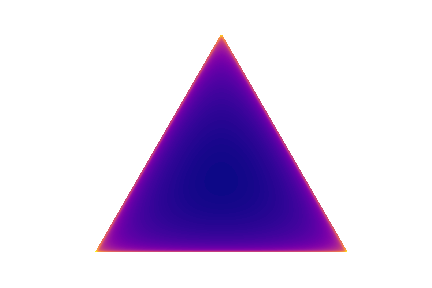
\includegraphics[width=\textwidth]{dir0995.png}
\caption*{$\lambda_\text{temp}=0.995$}
\end{minipage}
\hfill
 \begin{minipage}[t]{.3\textwidth}
   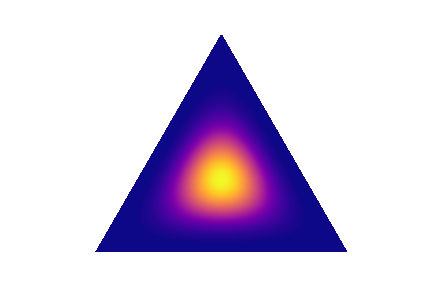
\includegraphics[width=\textwidth]{dir5.png}
\caption*{$\lambda_\text{temp}=5.0$}
\end{minipage}

\end{figure}

\end{frame}




\begin{frame}{Репараметризация}
\footnotesize
\begin{block}{Определение} Случайную величину  $\psi$ с распределением $q$ с параметрами $\teta_\psi$ назовем репараметризованной через случайную величину $\varepsilon$, чье распределение не зависит от параметров $\teta_\psi$, если:
\[
   \psi = g(\varepsilon, \teta_\psi)
\]
где  $g$ --- некоторая непрерывная функция.
\end{block}

\textbf{Пример}
\[
    \E_{\qw} \log~\LL=  \int_{\w} \log~\LL \qw d\w.
\]
Продифференцируем по параметрам $\tetaw$:
\[
 \nabla_{\tetaw} \E_{\qw} \log \LL = 
\int_{\w}  \log \LL \nabla_{\tetaw}\qw d\w.
\]

Пусть возможна репараметризация:
$
    \w = \mathbf{g}(\boldsymbol{\varepsilon}, \tetaw).
$ 
Тогда:
\[
 \nabla_{\tetaw} \E_{\q} \log \LL = \nabla_{\tetaw} \E_{\boldsymbol{\varepsilon}} \log \LL [][][\mathbf{g}(\boldsymbol{\varepsilon})] =
\]
\[= \int_{\boldsymbol{\varepsilon}}\nabla_{\tetaw} \log\LL [][][\mathbf{g}(\boldsymbol{\varepsilon})] p(\boldsymbol{\varepsilon}) d\boldsymbol{\varepsilon}=\E_{\boldsymbol{\varepsilon}} \nabla_{\tetaw} \log\LL [][][\mathbf{g}(\boldsymbol{\varepsilon})].\]
\textbf{Проблема:} не всегда просто найти $\mathbf{g}$.
\end{frame}


\begin{frame}{Implicit Reparameterization Gradients}
Пусть $\mathbf{g}^{-1}$ --- обратная функция к функции $\mathbf{g}$.
\textbf{Формула полной производной:}
\[
    \nabla^{\text{total}} f(x_1,\dots,x_n) = \sum \frac{\partial{f}}{\partial{x_i}}.
\]

Применяем к равенству:
\[
    \mathbf{g}^{-1}(\w) = \varepsilon.
\]

Получаем равенстнво:
\[
    \nabla_{\tetaw} \mathbf{g}(\varepsilon, \tetaw) = -\left(\nabla_{\w} \mathbf{g}^{-1}(\w) \right)^{-1} \nabla_{\tetaw} \mathbf{g}^{-1}(\w).
\]
\textbf{Универсальная функция стандартизации:}
\[
    \mathbf{g}^{-1}(\w) = F(\w) \sim \mathcal{U}(0,1),
\]
можно использовать методы сэмплирования типа MCMC.
\end{frame}



\begin{frame}{Logit-Normal}
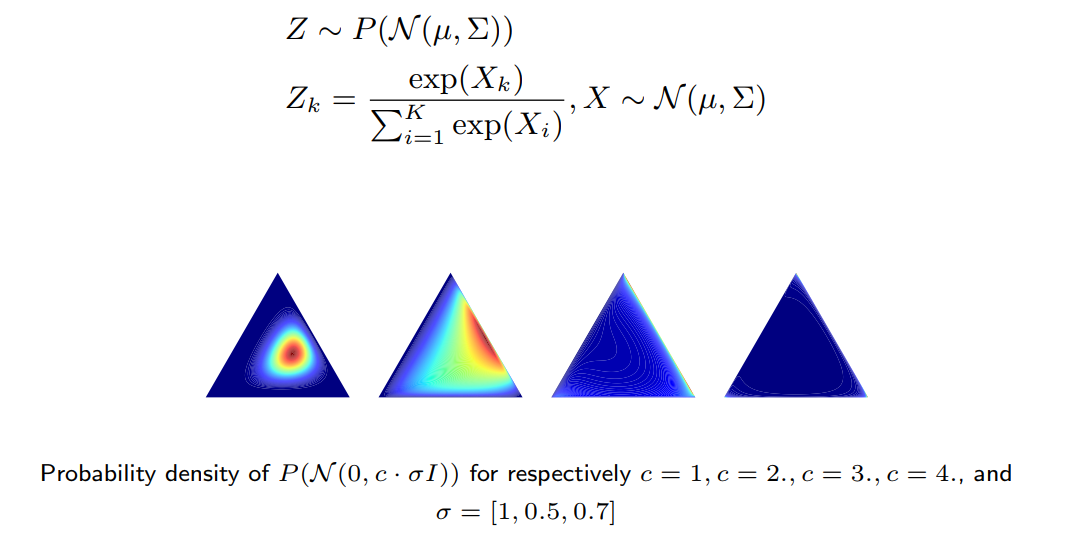
\includegraphics[width=0.9\textwidth]{logn.png}
\begin{centering}
[Источник: Deep Generative Models, http://stat.columbia.edu]
\end{centering}
\end{frame}



\begin{frame}{Априорное распределение на структуре модели}
Каждая точка на симплексе задает модель.


\textbf{Распределение Гумбель-софтмакс: }$\textcolor{red}{\boldsymbol{\Gamma}\sim \text{GS}(\mathbf{s}, \lambda_\text{temp})}$\\
\begin{figure}
 \begin{minipage}[t]{.2\textwidth}
        \centering
\begin{tikzpicture}[%
x={(1.7cm,0cm)},
y={(0cm,1.7cm)},
]

\coordinate (A) at (0,0); 
\coordinate (B) at (1,0) ;
\coordinate (C) at (0.5,0.86); 

%Ecken
\node[circle,scale=0.5,fill=black,draw=black](Ap) at (0,0){};
\node[circle,scale=0.5,fill=black,draw=black](Bp) at (1,0){};
\node[circle,scale=0.5,fill=black,draw=black](Cp) at (0.5,0.86){};

%Kanten
\draw[] (A)
-- (B)  node[midway, below]{}
-- (C)      node[midway, right]{}
-- (A)  node[midway, left]{};

\end{tikzpicture}
\caption*{$\lambda_\text{temp}\to0$}
\end{minipage}
\hfill
 \begin{minipage}[t]{.2\textwidth}
   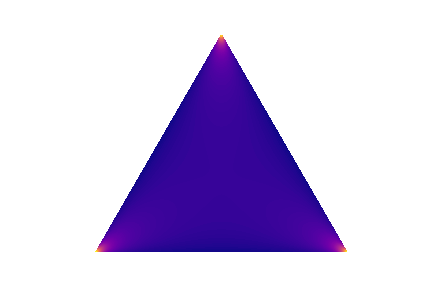
\includegraphics[width=\textwidth]{gs0995.png}
\caption*{$\lambda_\text{temp}=0.995$}
\end{minipage}
\hfill
 \begin{minipage}[t]{.2\textwidth}
   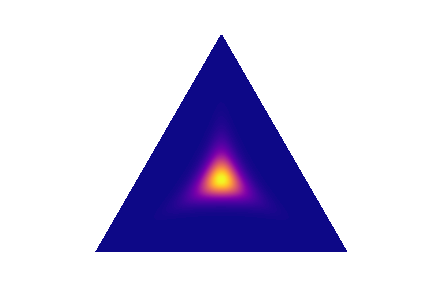
\includegraphics[width=\textwidth]{gs5.png}
\caption*{$\lambda_\text{temp}=5.0$}
\end{minipage}

\end{figure}

\textbf{Распределение Дирихле: }$\textcolor{red}{\boldsymbol{\Gamma}\sim \text{Dir}(\mathbf{s}, \lambda_\text{temp})}$\\
\begin{figure}
 \begin{minipage}[t]{.2\textwidth}
        \centering
\begin{tikzpicture}[%
x={(1.7cm,0cm)},
y={(0cm,1.7cm)},
]

\coordinate (A) at (0,0); 
\coordinate (B) at (1,0) ;
\coordinate (C) at (0.5,0.86); 

%Ecken
\node[circle,scale=0.5,fill=black,draw=black](Ap) at (0,0){};
\node[circle,scale=0.5,fill=black,draw=black](Bp) at (1,0){};
\node[circle,scale=0.5,fill=black,draw=black](Cp) at (0.5,0.86){};

%Kanten
\draw[] (A)
-- (B)  node[midway, below]{}
-- (C)      node[midway, right]{}
-- (A)  node[midway, left]{};

\end{tikzpicture}
\caption*{$\lambda_\text{temp}\to0$}
\end{minipage}
\hfill
 \begin{minipage}[t]{.2\textwidth}
   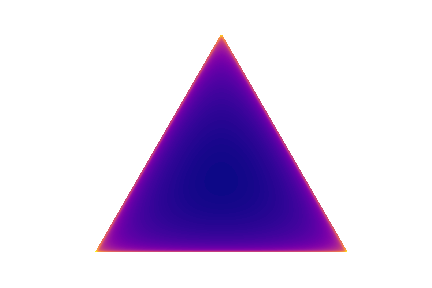
\includegraphics[width=\textwidth]{dir0995.png}
\caption*{$\lambda_\text{temp}=0.995$}
\end{minipage}
\hfill
 \begin{minipage}[t]{.2\textwidth}
   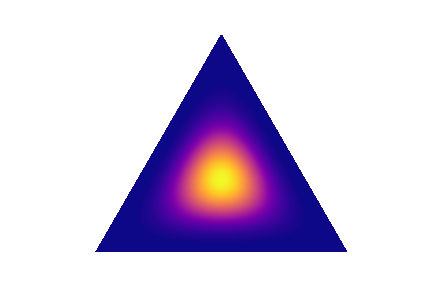
\includegraphics[width=\textwidth]{dir5.png}
\caption*{$\lambda_\text{temp}=5.0$}
\end{minipage}

\end{figure}

\end{frame}


\begin{frame}{Обобщающая задача оптимизации}
Какие требования можно выдвинуть к ``хорошей'' функции оптимизации?
\begin{enumerate}
\item При некоторых значениях метапараметров функция должна приближать \textcolor{blue}{метод максимального правдоподобия}.
\item При некоторых значениях метапараметров функция должна штрафовать \textcolor{red}{излишне сложные модели.}
\item При некоторых значениях метапараметров функция должна приближать обоснованность модели.
\item При некоторых значениях метапараметров функция должна позволять \textcolor{olive}{переходить между оптимальными структурами модели.}
\item Функции потерь и валидации должны быть непрерывны по метапараметрам.
\item Область определения функции должна быть нетривиальна.
\end{enumerate}
\end{frame}


\begin{frame}{Вероятностная модель}


\begin{columns}
\begin{column}{0.4\textwidth}
\textbf{Базовая модель:} %https://www.microsoft.com/en-us/research/wp-content/uploads/2016/02/bishop-variational-icann-98.pdf
\begin{itemize}
\item \textbf{параметры} модели\\ $\textcolor{red}{\mathbf{w} \sim \mathcal{N}(0, \alpha^{-1})},$
\item \textbf{гиперпараметры} модели $\mathbf{h} = [\alpha].$
\end{itemize}
\begin{figure}
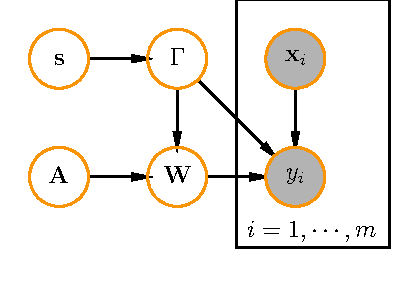
\includegraphics[width=\textwidth]{simple_plate_concrete.pdf}
\end{figure}
\end{column}
\begin{column}{0.6\textwidth}
\textbf{Предлагаемая модель: }
\begin{itemize}
\item \textbf{параметры} модели\\ $\textcolor{red}{\mathbf{w}_r^{j,k} \sim \mathcal{N}(0, (\gamma_{r}^{j,k})^2 (\mathbf{A}_r^{j,k})^{-1})},$
$\mathbf{A}_r^{j,k}$ --- диагональная матрица параметров, соответствующих базовых функций $\mathbf{g}_r^{j,k}$,
\\$\textcolor{olive}{(\mathbf{A}_r^{j,k})^{-1} \sim \text{inv-gamma}(\lambda_1,\lambda_2)},$

\item \textbf{структурные параметры} модели \\$\boldsymbol{\Gamma} = \{\boldsymbol{\gamma}^{j,k}, (j,k) \in E\},$ \\$\textcolor{red}{\boldsymbol{\gamma}^{j,k} \sim \text{GS}(\mathbf{s}^{j,k}, \lambda_\text{temp})},$ 
\item \textbf{гиперпараметры} модели $\mathbf{h} = [\text{diag}(\mathbf{A}), \mathbf{s} ],$
\item \textbf{метапараметры} $\lambda_1,\lambda_2,\lambda_\text{temp}$.
\end{itemize}

\end{column}

\end{columns}

%

\end{frame}


\begin{frame}{Предлагаемая задача оптимизации}

\footnotesize
\begin{columns}
\begin{column}{0.8\textwidth}
\begin{block}{Теорема [Бахтеев, 2018]}
Пусть функции потерь и валидации $L,Q$ являются непрерывно-дифференцируемыми на компакте $U$.
Тогда следующая задача является обобщающей на $U$.
\[
\mathbf{h}^{*} = \argmax_{\mathbf{h}} Q = 
\]
\[
= \textcolor{blue}{\lambda_\text{likelihood}^\text{Q}\mathsf{E}_{{q}^{*}} \text{log}~{p(\mathbf{y} | \mathbf{X}, \mathbf{w},\boldsymbol{\Gamma}, \mathbf{h}, \lambda_\text{temp}, \mathbf{f})}}
 -\]
\vspace{-0.3cm}
\[- \textcolor{red}{^\text{prior}_\text{Q}\text{D}_{KL}\bigl( q^{*}(\mathbf{w}, \boldsymbol{\Gamma}) || p(\mathbf{w}, \boldsymbol{\Gamma} |\mathbf{h}, \lambda_{\text{temp}},\mathbf{f}) \bigr)}  -\]
\vspace{-0.3cm}
\[
 - \textcolor{olive}{\sum_{p' \in \mathfrak{P}, \lambda \in \boldsymbol{\lambda}^\text{struct}_\text{Q}} \lambda\text{D}_{KL}(\boldsymbol{\Gamma} | p')+ \text{log}p(\mathbf{h}|\mathbf{f})}, 
\]
где 
\[
\tag{$L^{*}$}
{q}^{*} = \argmax_{q} L = 
\textcolor{blue}{\mathsf{E}_q \text{log}~{p(\mathbf{y} | \mathbf{X}, \mathbf{w}, \boldsymbol{\Gamma}, \mathbf{h}, \lambda_{\text{temp}}, \mathbf{f})}}
\]
\vspace{-0.3cm}
\[- \textcolor{red}{^\text{prior}_\text{L}\text{D}_{KL}\bigl( q^{*}(\mathbf{w}, \boldsymbol{\Gamma}) || p(\mathbf{w}, \boldsymbol{\Gamma} |\mathbf{h}, \lambda_{\text{temp}},\mathbf{f}) \bigr)}.
\]
\end{block}
%$\lambda^\text{likelihood}_\text{L}, \lambda^\text{prior}_\text{L}, \lambda^\text{prior}_\text{Q},  \boldsymbol{\lambda}_{\text{struct}}^Q, \lambda_{\text{temp}}$ и параметры распределений $\mathbf{P}$ --- метапараметры оптимизации.\\
Оптимизационная задача обобщает алгоритмы оптимизации: оптимизация правдоподобия и обоснованности, последовательное увеличение и снижение сложности модели, полный перебор структуры.
\end{column}
\begin{column}{0.2\textwidth}
\begin{figure}
\centering
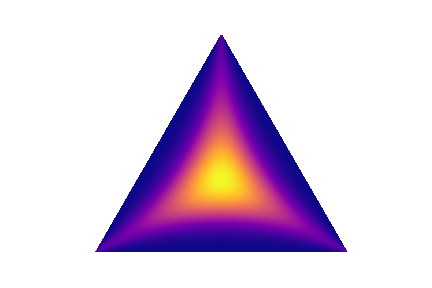
\includegraphics[width=0.75\textwidth]{combinations_1.png}
\end{figure}
\vspace{-0.2cm}
$ \textcolor{olive}{\boldsymbol{\lambda}_{\text{struct}}^Q=[0;0;0].}$
\begin{figure}
\centering
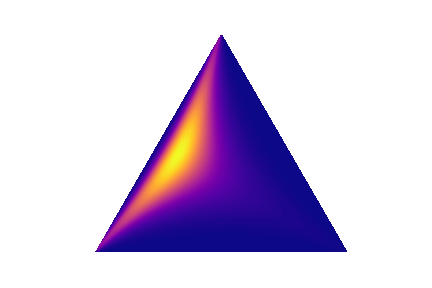
\includegraphics[width=0.75\textwidth]{combinations_2.png}
\end{figure}
\vspace{-0.2cm}
$ \textcolor{olive}{\boldsymbol{\lambda}_{\text{struct}}^Q=[1;0;0].}$
\begin{figure}
\centering
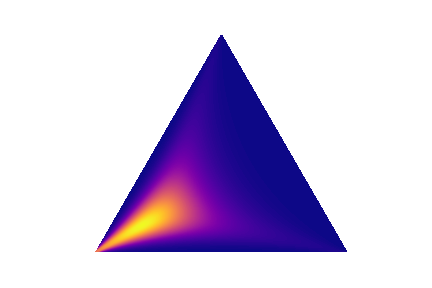
\includegraphics[width=0.75\textwidth]{combinations_3.png}
\end{figure}
\vspace{-0.2cm}
$ \textcolor{olive}{\boldsymbol{\lambda}_{\text{struct}}^Q=[1;1;0].}$
\end{column}
\end{columns}
\end{frame}


\begin{frame}{Свойства задачи оптимизации}
\begin{itemize}
\item Коэффициенты при ${D}_\text{KL}$ контролируют эффективный размер выборки.
\item При $\lamCQ  = \lamCL = \lamLL = 1$ --- вариационная оценка.
\item При $\frac{\lamCQ}{\lamLL} = \lamCL$ --- сводится к одноуровневой оптимизации.
\item При $\lamCQ = 0, \lamCL = 1$ --- вариационная оценка обоснованности, при гиперпараметрах, доставляющих максимум правдоподобия.
\item При $\lamCL = 0$ --- метод максимального правдоподобия.
\end{itemize}

\begin{block}{Утверждение}
Пусть $\textcolor{olive}{\boldsymbol{\lambda}^Q_{\text{struct}}} = \bf 0$.
Пусть  $\teta_1, \teta_2, \h_1, \h_2$ --- результаты оптимизации при разных значениях гиперпараметров $\textcolor{red}{{\lamCQ}_1,{\lamCQ}_2, {\lamCQ}_1>{\lamCQ}_2}$ на компакте $U$.
Пусть функция $\Val$ является вогнутой на $U$ при $\textcolor{red}{{\lamCQ}_2}$.
Тогда:
\footnotesize
\vspace{-0.2cm}
\[
    C_p(\teta_1|\Uh, \lam_1) - C_p(\teta_2|\Uh, \lam_2)  < \frac{\lamCL }{{\lamCQ}_2} ({\lamCQ}_2- \lamCL) C,
\]
где $C$ --- некоторая константа.
\end{block}


\end{frame}

\begin{frame}{Пример}
Подмодели: обобщено-линейная с одним признаком, с 11 признаками, константа.
\begin{center}
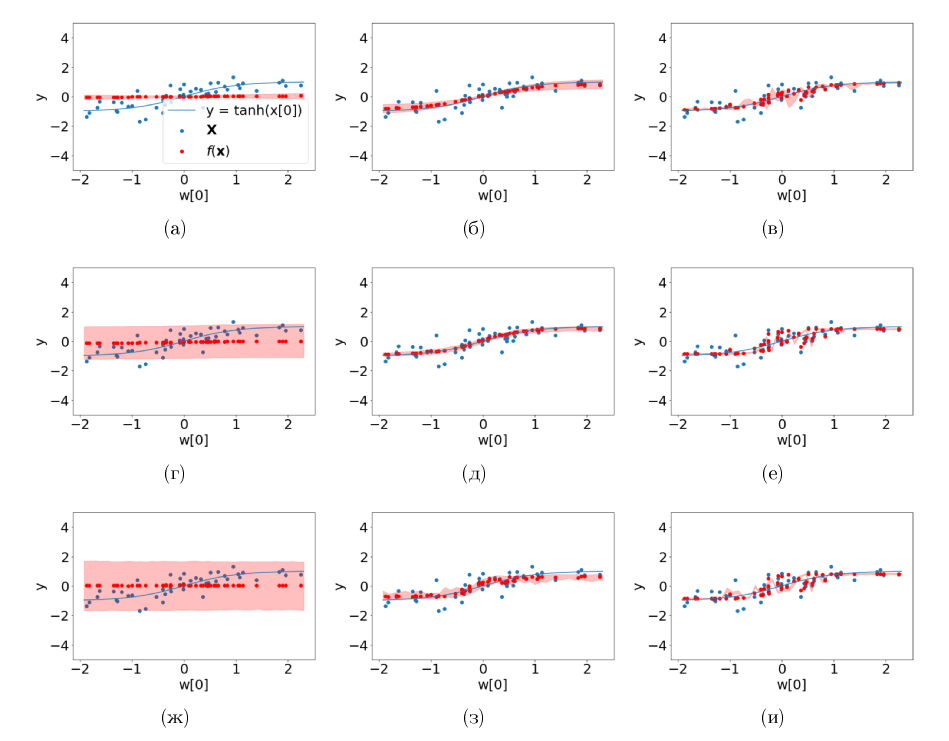
\includegraphics[width=0.66\textwidth]{example.png}
\end{center}
\end{frame}

\begin{frame}{Пример}
Подмодели: обобщено-линейная с одним признаком, с 11 признаками, константа.
\begin{center}
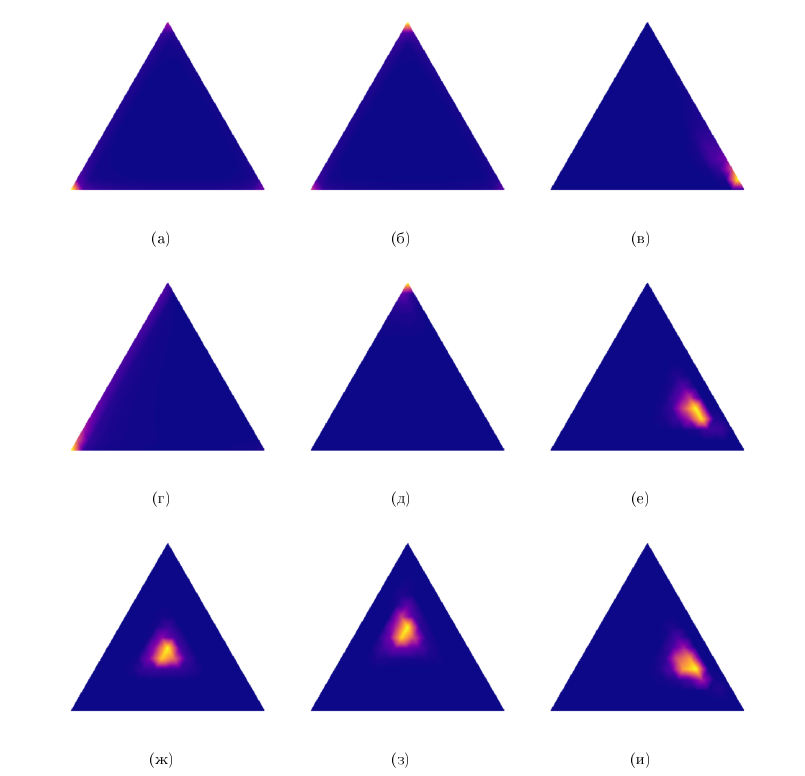
\includegraphics[width=0.44\textwidth]{example2.png}
\end{center}
\end{frame}



\begin{frame}
\frametitle{Список источников}
\begin{itemize}
\item MacKay, David JC. "Bayesian nonlinear modeling for the prediction competition." ASHRAE transactions 100.2 (1994): 1053-1062.
\item Graves, Alex. "Practical variational inference for neural networks." Advances in neural information processing systems. 2011.
\item Karaletsos, Theofanis, and Gunnar Rätsch. "Automatic relevance determination for deep generative models." arXiv preprint arXiv:1505.07765 (2015).
\item Cortes, Corinna, et al. "Adanet: Adaptive structural learning of artificial neural networks." Proceedings of the 34th International Conference on Machine Learning-Volume 70. JMLR. org, 2017.
\item Zoph, Barret, and Quoc V. Le. "Neural architecture search with reinforcement learning." arXiv preprint arXiv:1611.01578 (2016).
\item Zoph, B., Vasudevan, V., Shlens, J. and Le, Q.V., 2018. Learning transferable architectures for scalable image recognition
\item Liu, Hanxiao, Karen Simonyan, and Yiming Yang. "Darts: Differentiable architecture search." arXiv preprint arXiv:1806.09055 (2018).
\end{itemize}
\end{frame}

\begin{frame}
\frametitle{Список источников}
\begin{itemize}

\item Figurnov M., Mohamed S., Mnih A. Implicit reparameterization gradients //Advances in Neural Information Processing Systems. – 2018. – С. 441-452.
\item http://stat.columbia.edu/{\textasciitilde}cunningham/teaching/GR8201/STAT\\\_GR8201\_2019\_SPRG\_slides\_lec03.pdf
\item Jang, Eric, Shixiang Gu, and Ben Poole. "Categorical reparameterization with gumbel-softmax." arXiv preprint arXiv:1611.01144 (2016).
\item Maddison, Chris J., Andriy Mnih, and Yee Whye Teh. "The concrete distribution: A continuous relaxation of discrete random variables." arXiv preprint arXiv:1611.00712 (2016).
\end{itemize}
\end{frame}



\begin{frame}{ДЗ: выбор задания}
\textbf{Дедлайн: 27 ноября, 0 часов.}\\~\\

\texttt{ from zlib import crc32}\\~\\
\texttt{theory = crc32('фамилия кириллицей'.lower().encode('utf-8'))\%2+1}\\~\\
\texttt{practice = 1}\\~\\

Задания заливаются на github:
\textit{https://github.com/Intelligent-Systems-Phystech/model\_selection/фамилия латиницей}\\

\end{frame}

\begin{frame}{ДЗ: теория}
\textbf{Формат: tex + pdf.}

\textbf{Задание 1:}

Доказать, что при устремлении параметра температуры к бесконечности, плотность Gumbel-Softmax концентрируется в центре симплекса.

(за формулами Gumbel-Softmax обращаться к оригинальным статьям, Jang et al., Maddison et al.).
\end{frame}



\begin{frame}{ДЗ: теория}
\textbf{Формат: tex + pdf.}

\textbf{Задание 2:}
Доказать утверждение:
\begin{block}{утверждение}
Пусть задан компакт $U = \Uh \times \Uteta$ и  $\lamS=\mathbf{0}$. Пусть решение задачи
\[
\min_{\h \in \Uh} \KL{\q[\teta_2]}{p(\w, \Gam|\h)}
\]
 является единственным для некоторых ${\lamCQ}_1, {\lamCQ}_2, {\lamCQ}_1 > {\lamCQ}_2$ на $U$ при некоторых фиксированных $\lamLL, \lamCL, \lamT$.
Пусть также решения задач из слайда 20 являются единственными на $U$ при ${\lamCQ}_1, {\lamCQ}_2$ и $\lamLL, \lamCL, \lamT$.
Тогда справедливо следующее неравенство:
\[
    \KL{\q[\teta_1]}{p(\w, \Gam|\h_1)}  <   \KL{\q[\teta_2]}{p(\w, \Gam|\h_2)},
\]
где $\h_1, \teta_1,$ $\h_2, \teta_2$  --- решения задачи  при ${\lamCQ}_1, {\lamCQ}_2$,
$$
\teta_1 = \teta^{*}(\h_1), \quad  \teta_2 = \teta^{*}(\h_2).$$

\end{block}


\end{frame}

\begin{frame}{ДЗ: практика}
\textbf{Формат: ipynb.}
Реализовать визуализация зависимоссти распределения Gumbel-Softmax от температуры.

Пример для распределения Дирихле:
http://blog.bogatron.net/blog/2014/02/02/visualizing-dirichlet-distributions/

При оценивании будут учитываться аккуратность кода ноутбуков и наглядность примера.\\~\\
Пример должен быть выполнен на  \textbf{простых} игрушечных синтетических данных.
\end{frame}

\end{document}
